The simulation of eight different selfish mining strategies with five distinct distributions of computational power provides a reasonable outcome to argue the two research questions of the thesis.

\section{RQ1}

\textit{Do the simulations of selfish mining with the proposed software solutions show an increase of the total and relative gain for the selfish miner compared to the normal, honest mining behaviour?}

The simulation showed that the relative share of mining rewards obtained with selfish mining is higher compared to the honest mining if the miner has over 40\% of mining power and conducts a satisfactory selfish mining strategy.
To the satisfactory strategies, all strategies expect the combination lead stubborn and equal-fork stubborn (\textit{L, F}) and selfish mining with all three modifications (\textit{L, F T\textsubscript{1}}) can be counted.
The curves of the six good-performing strategies depicted in figure \ref{fig:accepted_blocks_selfish} show all a similar behaviour where their relative gain increases non-linearly with a higher computational share.
Out of these six strategies, the most promising strategies are normal selfish mining (\textit{S}) and equal-fork stubbornness (\textit{F}).
When these two strategies are applied, the selfish miner can create 49.1\%/50\% of the blocks of the longest chain even though its share of the mining power is only 45\%.

In all cases where the selfish miner has a low share of computational power, the results of the simulation show that the selfish mining does not increase the relative gain.
For example, when the selfish miner has 15\% of the mining power in the network only about 5\% of its blocks end up in the longest chain.
Even if the selfish miner has 37.5\% share of the computational power the most advantageously strategy (\textit{S}) only creates 32.4\% blocks of the longest chain.
The worst performing mining strategy in the scenario where the selfish miner has 37.5\% is the strategy with all three modifications (\textit{L, F, T\textsubscript{1}}) generating only 22.7\% of the accepted blocks.

Concluding it can be said that with the defined simulation scenario and the proposed software solutions only for a very high computational share an increase of the relative gain could be observed.
For all scenarios where the selfish miner has less than 40\% percent, the miner would earn relatively more by behaving honestly.

\section{RQ2}

\textit{How do the obtained results of the simulation match the outcome of previous research in the area of selfish mining?}

When comparing the outcome from the simulations with recent studies, it first needs to be considered that with the introduced simulation framework the outcome of the block races cannot be defined directly, as it is the case in previously used types of simulation.
Instead, the block races happen naturally during the execution of a scenario.
With the used simulation scenario and implementation of the selfish proxy, it is likely that the parameter $\gamma$, denoting if an honest node extends the private chain during a block race, is almost zero.
This assumption is based on the configured network topology and the implementation of the selfish proxy.
In the scenario, a fully connected network topology is used where each connection has the same latency.
Hence, when a node finds a block, it sends the block to all nodes directly.
Then it is unlikely that the selfish node can advertise its block faster to other nodes using the same connections before the honest nodes have already adopted to the new public tip.
The implementation of the selfish proxy further worsens the position of the selfish miner when trying to match a competing block during a block race.
The proxy which eclipses the private node does not implement the fast block propagation mechanism \textit{compact blocks}.
Instead, the proxy uses the standard but slower block propagation technique to receive and send blocks.
Thus, the proxy receives and sends blocks slower than the rest of the network.

Assuming that the probability of the selfish miner to win a block race is very low, the attained results match the outcome of previous research closely.
In figure \ref{fig:eyal_results} the red line shows the relative revenue of the selfish miner conducting normal selfish mining when it is not able to win any block race \cite{eyal2014majority}.
The curve shows the same concave course as in figure \ref{fig:accepted_blocks_selfish} underlining that with an increase of the computational share the efficiency of the selfish mining is amplified.
Moreover, the selfish miner achieved more relative revenue compare to the honest miner with about 36\% of the mining power, similar to the slightly worse results of 40\% showed in chapter \ref{chap:results}.
Comparable outcomes for the selfish mining without any modification were produced in other recent research \cite{nayak2016stubborn, sapirshtein2016optimal}.

\begin{figure}[t]
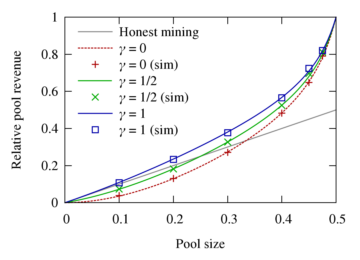
\includegraphics[width=8cm]{eyal_results}
\centering
\caption{Results obtained by \cite{eyal2014majority} with normal selfish mining}
\label{fig:eyal_results}
\end{figure}

In figure \ref{fig:nayak_results_1} optimal selfish mining strategies including stubborn modifications from the research of \cite{nayak2016stubborn} are shown.
In the case, where the selfish miner loses all block races, the honest behaviour is the most profitable strategy until a computational share of 34\% is reached.
Afterwards, the most advantageous mining strategy is trail stubbornness (\textit{T\textsubscript{1}}) up to a computational share of 45\%.
From 45\% to 50\% the dominant strategy is trail stubborn in combination with equal-fork stubborn (\textit{T\textsubscript{1}, F}), but in many cases, the best strategy is not clear signalised by the black dots in the graphic.
The results of the optimal stubborn mining strategy by \cite{nayak2016stubborn} slightly differ to the outcome of the simulation from chapter \ref{chap:results}.
In the proposed simulation the best performing strategies were the normal selfish mining (\textit{S}) and equal-fork stubborn mining (\textit{F}) with trail stubbornness combined with equal-fork stubbornness (\textit{T\textsubscript{1}, F}) and trail stubbornness (\textit{T\textsubscript{1}}) being only the third and fourth most satisfactory strategy.

\cite{nayak2016stubborn} does not propose the actual ranking of different selfish strategies regarding their performance for a specific $\gamma$ but provides a comparison of the relative gain obtained by selfish mining and selfish mining with stubborn modifications.
On the assumption that $\gamma$ is zero, the relative gain achieved by using stubborn modifications over selfish mining is very low as shown in figure \ref{fig:nayak_results_2}.
Thus, also in the research of \cite{nayak2016stubborn}, the normal selfish mining forms a viable strategy comparable to the results obtained in the previous chapters.
Furthermore, figure \ref{fig:nayak_results_1} showed that between 45\% and 50\% the best strategy is not always known denoted by the black dots.
From that concludes, that in the case where all block races are won by the honest network, the optimal strategy is not identifiable, similar to the outcome from the proposed simulations where the four best strategies were 3\% apart.

\begin{figure}[t]
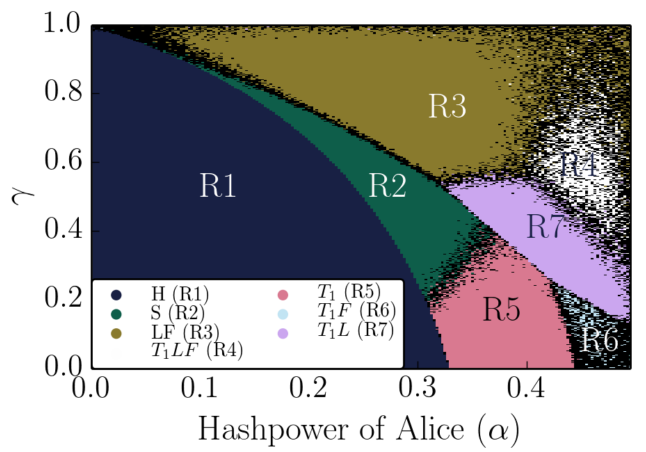
\includegraphics[width=8cm]{nayak_results_1}
\centering
\caption{Optimal stubborn mining strategies retrieved by \cite{nayak2016stubborn}}
\label{fig:nayak_results_1}
\end{figure}

Summarising the obtained simulations results are comparable to recent research even though the outcome of the simulation was slightly worse than results from previous research.
Regarding the best performing selfish mining strategies also the research of \cite{nayak2016stubborn} showed that differences in the case where $\gamma$ equals zero are subtle.
Nevertheless, both studies showed similar good performing selfish mining strategies.

\begin{figure}[t]
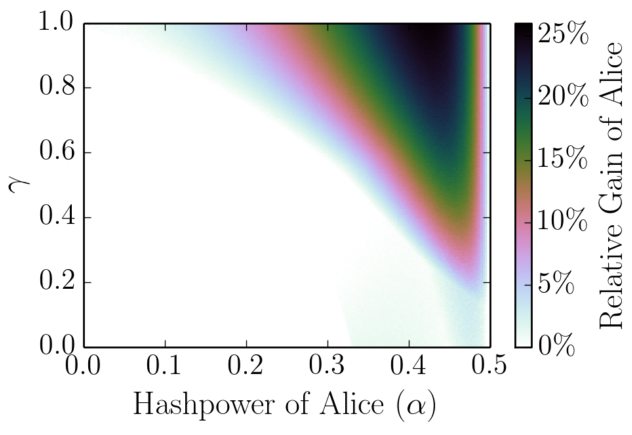
\includegraphics[width=8cm]{nayak_results_2}
\centering
\caption{Selfish mining compared to optimal stubborn mining strategies by \cite{nayak2016stubborn}}
\label{fig:nayak_results_2}
\end{figure}

\section{Profitability}

As previously evaluated selfish mining can increase the relative gain of the misbehaving miner, but the results of the simulations show further that the absolute amount of accepted blocks is lower as shown in figure \ref{fig:accepted_blocks_selfish}.
Hence, the selfish miner is earning less mining rewards even though its relative revenue is increasing.
The loss of profit is possible because the stale block rate increases during selfish mining, and thus, fewer blocks end up in the longest chain.
To still profit from the attack the miner would need to wait for the difficulty adjustment.
After the difficulty adjustment, the nodes in the network can find more blocks and hence, also the selfish miner can create more blocks.
Since selfish mining was never observed for such a long time and no research was conducted in this area, it is not clear if such a long attack would be successful \cite{nayak2016stubborn}.
